% summary.tex
% mainfile: perfbook.tex
% SPDX-License-Identifier: CC-BY-SA-3.0

\chapter{Looking Forward and Back}
\label{chp:Looking Forward and Back}
%
\Epigraph{History is the sum total of things that could have been avoided.}
	  {\emph{Konrad Adenauer}}

You have arrived at the end of this book, well done!
I~hope that your journey was a pleasant but challenging and worthwhile
one.

For your editor and contributors, this is the end of the journey to the
Second Edition, but for those willing to join in, it is also the start
of the journey to the Third Edition.
Either way, it is good to recap this past journey.

\Cref{chp:How To Use This Book} covered what this book is about, along
with some alternatives for those interested in something other than
low-level parallel programming.

\Cref{chp:Introduction} covered parallel-programming challenges and
high-level approaches for addressing them.
It also touched on ways of avoiding these challenges while nevertheless
still gaining most of the benefits of parallelism.

\Cref{chp:Hardware and its Habits} gave a high-level overview of multicore
hardware, especially those aspects that pose challenges for concurrent
software.
This \lcnamecref{chp:Hardware and its Habits} puts the blame for these
challenges where it belongs, very much on the laws of physics and rather
less on intransigent hardware architects and designers.
However, there might be some things that hardware architects and engineers
can do, and this \lcnamecref{chp:Hardware and its Habits} discusses a few of
them.
In the meantime, software architects and engineers must do their part
to meet these challenges, as discussed in the rest of the book.

\Cref{chp:Tools of the Trade}
gave a quick overview of the tools of the low-level concurrency trade.
\Cref{chp:Counting} then demonstrated use of those tools---and, more
importantly, use of parallel-programming design techniques---on the
simple but surprisingly challenging task of concurrent counting.
So challenging, in fact, that a number of concurrent counting algorithms
are in common use, each specialized for a different use case.

\Cref{cha:Partitioning and Synchronization Design} dug more deeply
into the most important parallel-programming design technique, namely
partitioning the problem at the highest possible level.
This \lcnamecref{cha:Partitioning and Synchronization Design} also
overviewed a number of points in this design space.

\Cref{chp:Locking} expounded on that parallel-programming workhorse
(and villain), locking.
This \lcnamecref{chp:Locking} covered a number of types of locking
and presented some engineering solutions to many well-known and
aggressively advertised shortcomings of locking.

\Cref{chp:Data Ownership} discussed the uses of data ownership, where
synchronization is supplied by the association of a given data item
with a specific thread.
Where it applies, this approach combines excellent performance and
scalability with profound simplicity.

\Cref{chp:Deferred Processing} showed how a little procrastination can
greatly improve performance and scalability, while in a surprisingly large
number of cases also simplifying the code.
A number of the mechanisms presented in this
\lcnamecref{chp:Deferred Processing}
take advantage of the ability of CPU caches to replicate read-only data,
thus sidestepping the laws of physics that cruelly limit the speed of
light and the smallness of atoms.
\Cref{chp:Data Structures} looked at concurrent data structures, with
emphasis on hash tables, which have a long and honorable history in
parallel programs.

\Cref{chp:Validation} dug into code-review and testing methods, and
\cref{chp:Formal Verification} overviewed formal verification.
Whichever side of the formal-verification/\-testing divide you might
be on, if code has not been thoroughly validated, it does not work.
And that goes at least double for concurrent code.

\Cref{chp:Putting It All Together} presented a number of situations
where combining concurrency mechanisms with each other or with other
design tricks can greatly ease parallel programmers' lives.
\Cref{sec:advsync:Advanced Synchronization} looked at advanced
synchronization methods, including lockless programming, IXacrl{nbs},
and parallel real-time computing.
\Cref{chp:Advanced Synchronization: Memory Ordering} dug into the
critically important topic of memory ordering, presenting techniques
and tools to help you not only solve memory-ordering problems, but
also to avoid them completely.
\Cref{chp:Ease of Use} presented a brief overview of the surprisingly
important topic of ease of use.

Last, but definitely not least, \cref{chp:Conflicting Visions of the Future}
expounded on a number of conflicting visions of the future, including
CPU-technology trends, transactional memory, hardware transactional
memory, use of formal verification in regression testing, and the
long-standing prediction that the future of parallel programming belongs
to functional-programming languages.

But now that we have recapped the contents of this Second Edition, how did
this book get started?

Paul's parallel-programming journey started in earnest in 1990, when
he joined Sequent Computer Systems, Inc.
Sequent used an apprenticeship-like program in which newly hired engineers
were placed in cubicles surrounded by experienced engineers, who mentored
them, reviewed their code, and gave copious quantities of advice on
a variety of topics.
A few of the newly hired engineers were greatly helped by the fact that
there were no on-chip caches in those days, which meant that
logic analyzers could easily display a given CPU's instruction stream
and memory accesses, complete with accurate timing information.
Of course, the downside of this transparency was that CPU core clock
frequencies were 100 times slower than those of the twenty-first
century.
Between apprenticeship and hardware performance transparency, these newly
hired engineers became productive parallel programmers within two or three
months, and some were doing ground-breaking work within a couple of years.

Sequent understood that its ability to quickly train new engineers in the
mysteries of parallelism was unusual, so it produced a slim volume that
crystalized the company's parallel-programming wisdom~\cite{SQNTParallel},
which joined a pair of groundbreaking papers that had been written a
few years earlier~\cite{Beck85,Inman85}.
People already steeped in these mysteries saluted this book and these
papers, but novices were usually unable to benefit much from them,
invariably making highly creative and quite destructive errors that
were not explicitly prohibited by either the book or the papers.\footnote{
	``But why on earth would you do \emph{that}???''
	``Well, why not?''}
This situation of course caused Paul to start thinking in terms of
writing an improved book, but his efforts during this time were limited
to internal training materials and to published papers.

By the time Sequent was acquired by IBM in 1999, many of the world's
largest database instances ran on Sequent hardware.
But times change, and by 2001 many of Sequent's parallel programmers
had shifted their focus to the Linux kernel.
After some initial reluctance, the Linux kernel community embraced
concurrency both enthusiastically and
effectively~\cite{SilasBoydWickizer2010LinuxScales48,McKenney:2012:BEP:2414729.2414734},
with many excellent innovations and improvements from throughout the
community.
The thought of writing a book occurred to Paul from time to time, but
life was flowing fast, so he made no progress on this project.

In 2006, Paul was invited to a conference on Linux scalability, and was
granted the privilege of asking the last question of panel of esteemed
parallel-programming experts.
Paul began his question by noting that in the 15~years from 1991 to 2006,
the price of a parallel system had dropped from that of a house to that
of a mid-range bicycle, and it was clear that there was much more room
for additional dramatic price decreases over the next 15~years
extending to the year 2021.
He also noted that decreasing price should result in greater familiarity
and faster progress in solving parallel-programming problems.
This led to his question:
``In the year 2021, why wouldn't parallel programming have become routine?''

The first panelist seemed quite disdainful of anyone who would ask such
an absurd question, and quickly responded with a soundbite answer.
To which Paul gave a soundbite response.
They went back and forth for some time, for example, the panelist's
sound-bite answer ``Deadlock'' provoked Paul's sound-bite response ``Lock
dependency checker''.

The panelist eventually ran out of soundbites, improvising a final
``People like you should be hit over the head with a hammer!''

Paul's response was of course ``You will have to get in line for that!''

Paul turned his attention to the next panelist, who seemed torn between
agreeing with the first panelist and not wishing to have to deal with
Paul's series of responses.
He therefore have a short non-committal speech.
And so it went through the rest of the panel.

Until it was the turn of the last panelist, who was someone you might have
heard of who goes by the name of Linus Torvalds.
Linus noted that three years earlier (that is, 2003), the initial version
of any concurrency-related patch was usually quite poor, having design
flaws and many bugs.
And even when it was cleaned up enough to be accepted, bugs still
remained.
Linus contrasted this with the then-current situation in 2006, in which
he said that it was not unusual for the first version of a concurrency-related
patch to be well-designed with few or even no bugs.
He then suggested that \emph{if} tools continued to improve, then \emph{maybe}
parallel programming would become routine by the year 2021.\footnote{
	Tools have in fact continued to improve, including fuzzers,
	lock dependency checkers, static analyzers, formal verification,
	memory models, and code-modification tools such as coccinelle.
	Therefore, those who wish to assert that year-2021
	parallel programming is not routine should refer to
	\cref{chp:Introduction}'s epigraph.}

The conference then concluded.
Paul was not surprised to be given wide berth by many audience members,
especially those who saw the world in the same way as did the first panelist.
Paul was also not surprised that a few audience members thanked him for
the question.
However, he was quite surprised when one man came up to say ``thank
you'' with tears streaming down his face, sobbing so hard that he could
barely speak.

You see, this man had worked several years at Sequent, and thus very
well understood parallel programming.
Furthermore, he was currently assigned to a group whose job it was to
write parallel code.
Which was not going well.
You see, it wasn't that they had trouble understanding his explanations
of parallel programming.

It was that they refused to listen to him \emph{at all}.

In short, his group was treating this man in the same way that the first
panelist attempted to treat Paul.
And so in that moment, Paul went from ``I should write a book some day''
to ``I will do whatever it takes to write this book''.
Paul is embarrassed to admit that he does not remember the man's name,
if in fact he ever knew it.

This book is nevertheless for that man.

\begin{figure}
\centering
\resizebox{3in}{!}{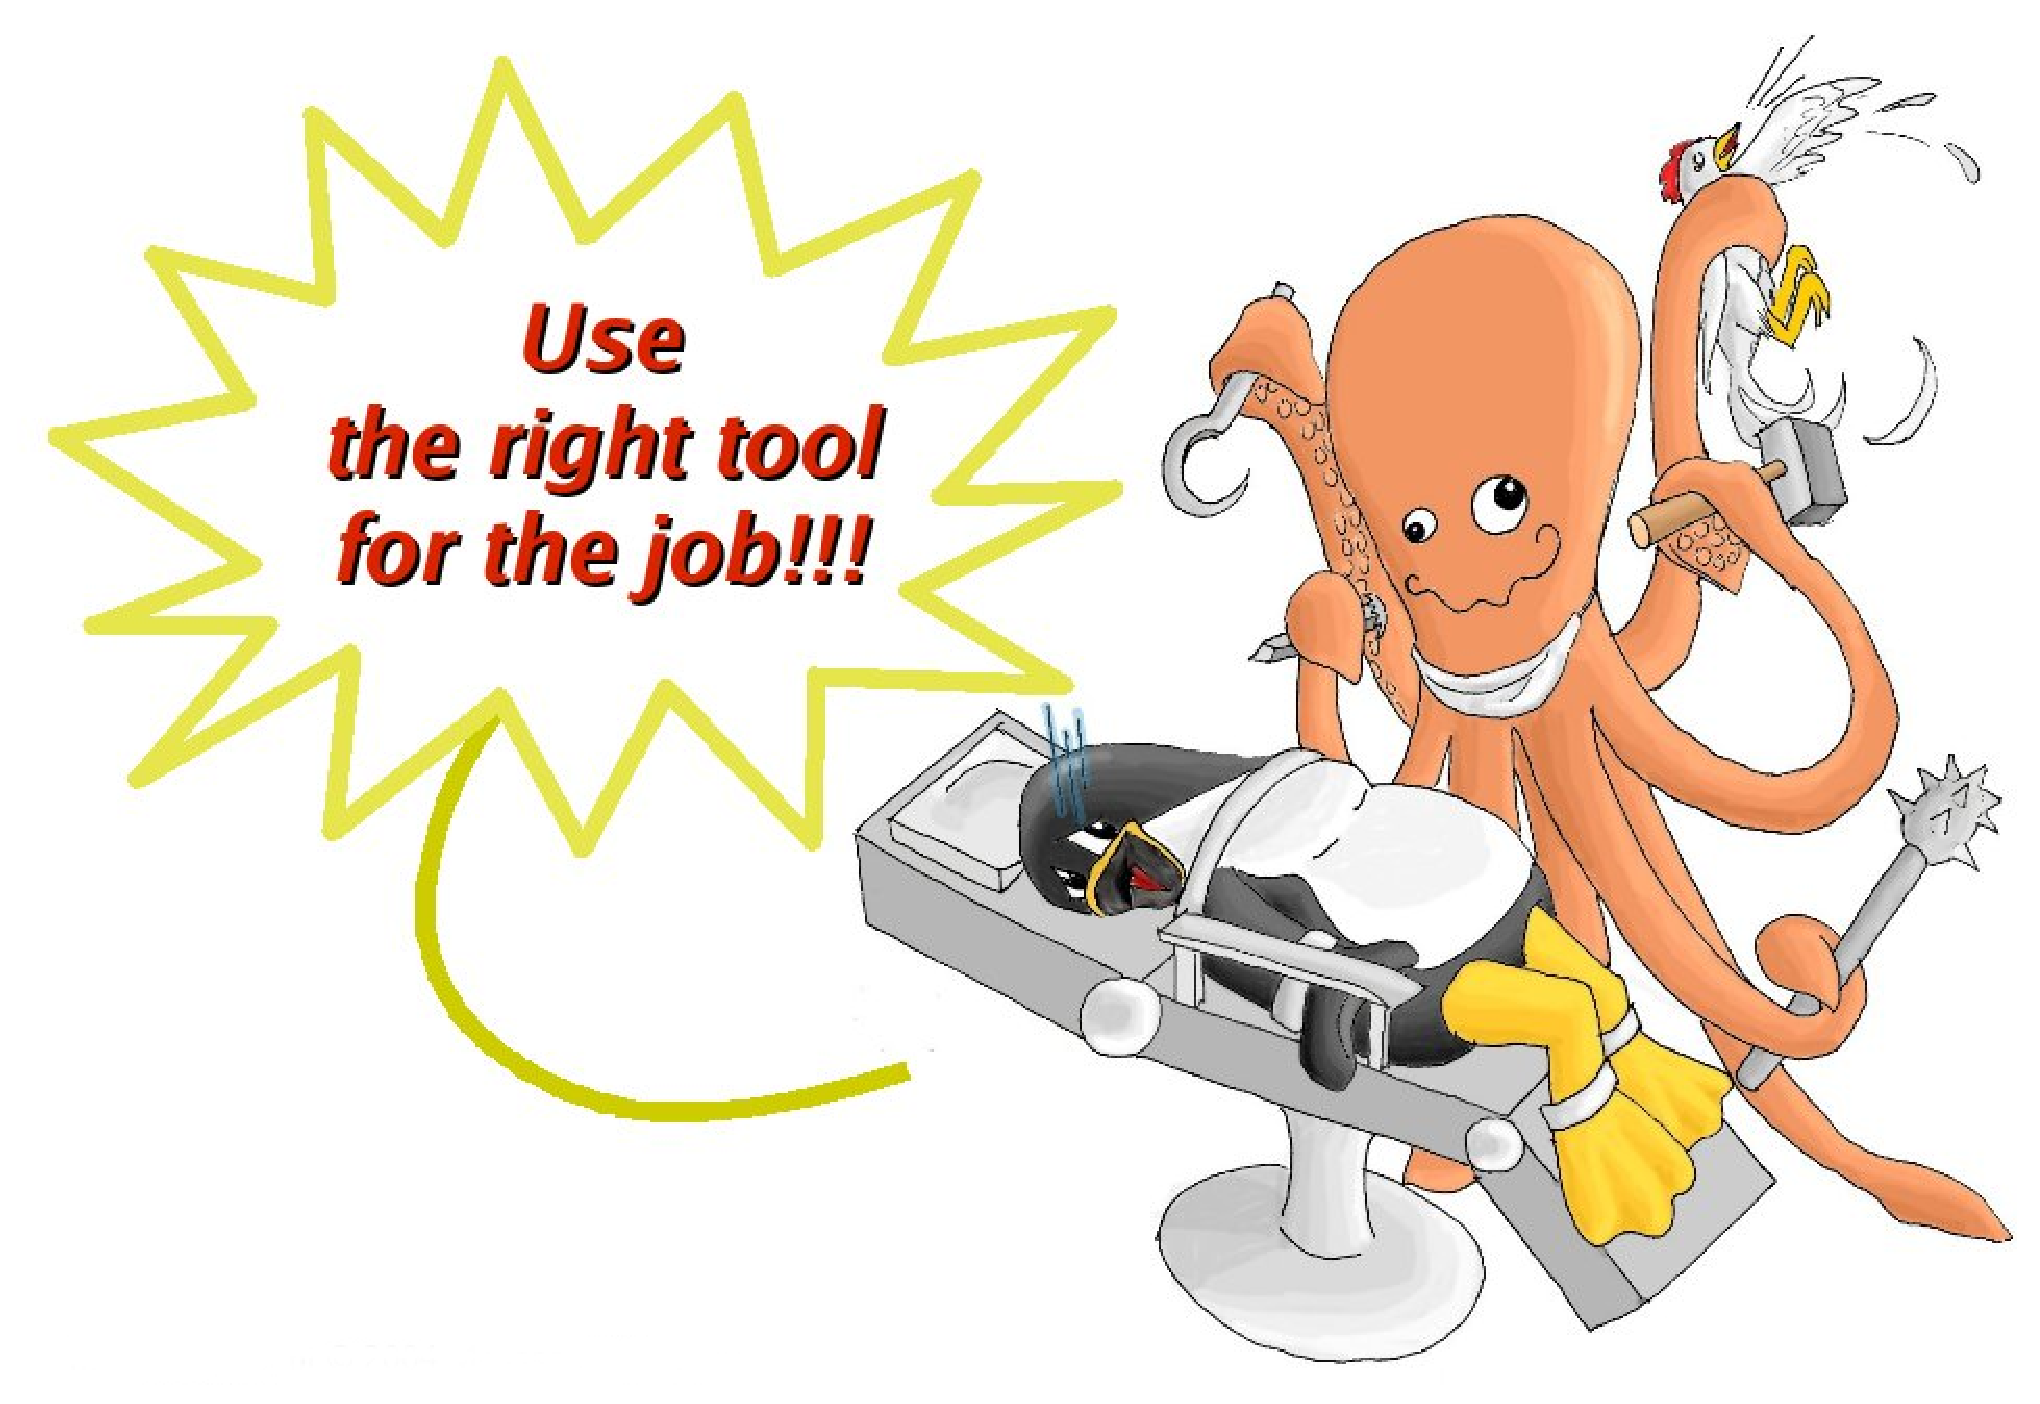
\includegraphics{cartoons/UseTheRightToolsBubble}}
\caption{The Most Important Lesson}
\ContributedBy{Figure}{fig:summary:The Most Important Lesson}{Melissa Broussard}
\end{figure}

And this book is also for everyone else who would like to add low-level
concurrency to their skillset.
If you remember nothing else from this book, let it be the lesson of
\cref{fig:summary:The Most Important Lesson}.

For the rest of us, when someone tries to show us a solution to pressing
problem, perhaps we should at the very least do them the courtesy of
listening!
